\documentclass[]{ctexbook}
\usepackage{lmodern}
\usepackage{amssymb,amsmath}
\usepackage{ifxetex,ifluatex}
\usepackage{fixltx2e} % provides \textsubscript
\ifnum 0\ifxetex 1\fi\ifluatex 1\fi=0 % if pdftex
  \usepackage[T1]{fontenc}
  \usepackage[utf8]{inputenc}
\else % if luatex or xelatex
  \ifxetex
    \usepackage{mathspec}
  \else
    \usepackage{fontspec}
  \fi
  \defaultfontfeatures{Ligatures=TeX,Scale=MatchLowercase}
\fi
% use upquote if available, for straight quotes in verbatim environments
\IfFileExists{upquote.sty}{\usepackage{upquote}}{}
% use microtype if available
\IfFileExists{microtype.sty}{%
\usepackage{microtype}
\UseMicrotypeSet[protrusion]{basicmath} % disable protrusion for tt fonts
}{}
\usepackage[b5paper,tmargin=2.5cm,bmargin=2.5cm,lmargin=3.5cm,rmargin=2.5cm]{geometry}
\usepackage{hyperref}
\PassOptionsToPackage{usenames,dvipsnames}{color} % color is loaded by hyperref
\hypersetup{unicode=true,
            pdftitle={R\_Dplyr\_minicourse},
            pdfauthor={陳柏銘},
            colorlinks=true,
            linkcolor=Maroon,
            citecolor=Blue,
            urlcolor=Blue,
            breaklinks=true}
\urlstyle{same}  % don't use monospace font for urls
\usepackage{natbib}
\bibliographystyle{plainnat}
\usepackage{longtable,booktabs}
\usepackage{graphicx,grffile}
\makeatletter
\def\maxwidth{\ifdim\Gin@nat@width>\linewidth\linewidth\else\Gin@nat@width\fi}
\def\maxheight{\ifdim\Gin@nat@height>\textheight\textheight\else\Gin@nat@height\fi}
\makeatother
% Scale images if necessary, so that they will not overflow the page
% margins by default, and it is still possible to overwrite the defaults
% using explicit options in \includegraphics[width, height, ...]{}
\setkeys{Gin}{width=\maxwidth,height=\maxheight,keepaspectratio}
\IfFileExists{parskip.sty}{%
\usepackage{parskip}
}{% else
\setlength{\parindent}{0pt}
\setlength{\parskip}{6pt plus 2pt minus 1pt}
}
\setlength{\emergencystretch}{3em}  % prevent overfull lines
\providecommand{\tightlist}{%
  \setlength{\itemsep}{0pt}\setlength{\parskip}{0pt}}
\setcounter{secnumdepth}{5}
% Redefines (sub)paragraphs to behave more like sections
\ifx\paragraph\undefined\else
\let\oldparagraph\paragraph
\renewcommand{\paragraph}[1]{\oldparagraph{#1}\mbox{}}
\fi
\ifx\subparagraph\undefined\else
\let\oldsubparagraph\subparagraph
\renewcommand{\subparagraph}[1]{\oldsubparagraph{#1}\mbox{}}
\fi

%%% Use protect on footnotes to avoid problems with footnotes in titles
\let\rmarkdownfootnote\footnote%
\def\footnote{\protect\rmarkdownfootnote}

%%% Change title format to be more compact
\usepackage{titling}

% Create subtitle command for use in maketitle
\newcommand{\subtitle}[1]{
  \posttitle{
    \begin{center}\large#1\end{center}
    }
}

\setlength{\droptitle}{-2em}
  \title{R\_Dplyr\_minicourse}
  \pretitle{\vspace{\droptitle}\centering\huge}
  \posttitle{\par}
  \author{陳柏銘}
  \preauthor{\centering\large\emph}
  \postauthor{\par}
  \predate{\centering\large\emph}
  \postdate{\par}
  \date{2018-04-26}

\usepackage{booktabs}

\usepackage{amsthm}
\newtheorem{theorem}{Theorem}[section]
\newtheorem{lemma}{Lemma}[section]
\theoremstyle{definition}
\newtheorem{definition}{Definition}[section]
\newtheorem{corollary}{Corollary}[section]
\newtheorem{proposition}{Proposition}[section]
\theoremstyle{definition}
\newtheorem{example}{Example}[section]
\theoremstyle{definition}
\newtheorem{exercise}{Exercise}[section]
\theoremstyle{remark}
\newtheorem*{remark}{Remark}
\newtheorem*{solution}{Solution}
\begin{document}
\maketitle

{
\hypersetup{linkcolor=black}
\setcounter{tocdepth}{2}
\tableofcontents
}
\listoftables
\listoffigures
\section*{課程規劃}
\addcontentsline{toc}{section}{課程規劃}

\subsection*{前言}
\addcontentsline{toc}{subsection}{前言}

Dplyr是R語言當中相當重要的資料處理套件,同時也是探索式資料分析的第一步。探索式資料分析是透過視覺化或敘述統計的方式,去觀察資料本身的特性或者變數與變數之間的關聯,以求對資料有更多的認識,看看是否有意外有趣的發現或者不符合常理的地方。當然也包含資料清理與建立必要變數的部分,必要時需要透過爬蟲或者引入第三方資料,才算完整。

資料處理做得好,整體的分析方向和後面的統計建模才會有意義且往對的道路前進,以避免不必要的時間、資源浪費。

\subsection*{課前要求}
\addcontentsline{toc}{subsection}{課前要求}

\begin{enumerate}
\def\labelenumi{\arabic{enumi}.}
\tightlist
\item
  安裝:R and R Studio Desktop: \url{https://www.rstudio.com}\\
\item
  \href{https://github.com/rstudio/cheatsheets/raw/master/data-transformation.pdf}{下載dplyr
  cheatsheet}
\item
  \href{連結}{填寫簽到單}
\end{enumerate}

\subsection*{課程大綱}
\addcontentsline{toc}{subsection}{課程大綱}

\begin{quote}
本課程將逐步介紹Dplyr常用的分析資料函數,會搭配dplyr
cheatsheet以及Help做講解,希望能夠在熟悉基本工具之後,甚至不需要這本電子書就能夠用效率的方式向Dplyr學習Dplyr。
\end{quote}

以下為講解的資料整理函數:

\begin{itemize}
\item
  認識資料基本資訊

  \begin{itemize}
  \tightlist
  \item
    \texttt{numeric} \texttt{interger} \texttt{character}
    \texttt{logic}:變數型態
  \item
    \texttt{head()}:變數型態
  \item
    \texttt{str()}:觀察整個資料集(dataset)結構
  \item
    \texttt{View()}:正式叫出資料集
  \end{itemize}
\item
  計算敘述統計量

  \begin{itemize}
  \tightlist
  \item
    \texttt{summarise}:單變量敘述統計量(平均數、標準差、四分為差、中位數)
  \item
    \texttt{covariance} \texttt{correlation}: 雙變量敘述統計量
  \end{itemize}
\item
  挑選適當的欄位
\item
  篩選適當觀察值
\item
  從既有變數產生新變數
\item
  分群分析(我還不會ungroup和group差別)
\item
  排序觀察值
\end{itemize}

\hypertarget{intro}{%
\section{Introduction}\label{intro}}

You can label chapter and section titles using \texttt{\{\#label\}}
after them, e.g., we can reference Chapter \ref{intro}. If you do not
manually label them, there will be automatic labels anyway, e.g.,
Chapter \ref{methods}.

Figures and tables with captions will be placed in \texttt{figure} and
\texttt{table} environments, respectively.

\begin{figure}

{\centering 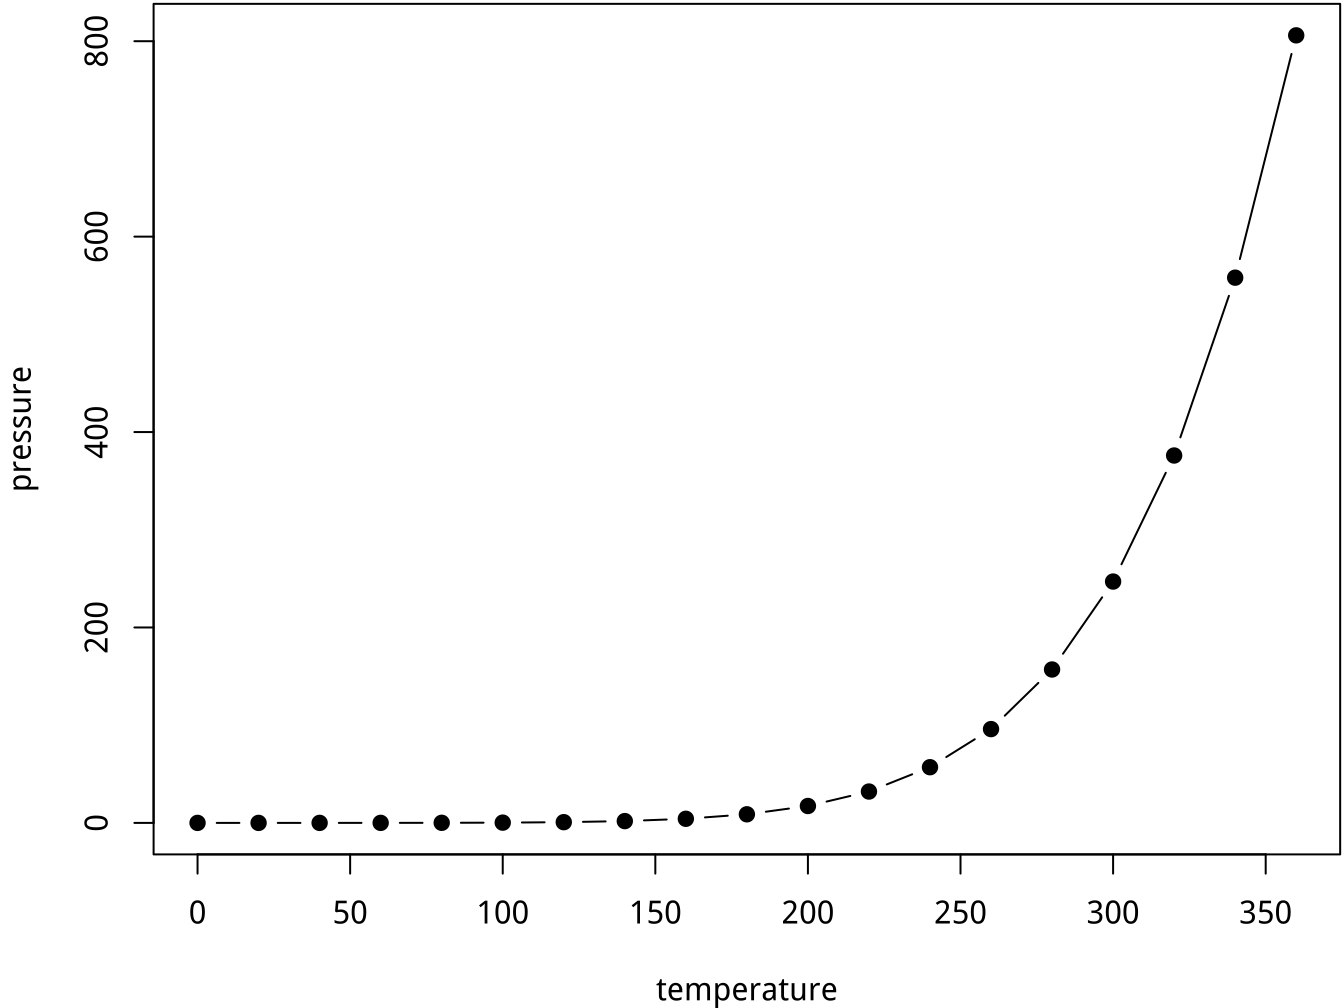
\includegraphics[width=0.8\linewidth]{Dplyr_minicourse_files/figure-latex/nice-fig-1} 

}

\caption{Here is a nice figure!}\label{fig:nice-fig}
\end{figure}

Reference a figure by its code chunk label with the \texttt{fig:}
prefix, e.g., see Figure \ref{fig:nice-fig}. Similarly, you can
reference tables generated from \texttt{knitr::kable()}, e.g., see Table
\ref{tab:nice-tab}.

\begin{table}

\caption{\label{tab:nice-tab}Here is a nice table!}
\centering
\begin{tabular}[t]{rrrrl}
\toprule
Sepal.Length & Sepal.Width & Petal.Length & Petal.Width & Species\\
\midrule
5.1 & 3.5 & 1.4 & 0.2 & setosa\\
4.9 & 3.0 & 1.4 & 0.2 & setosa\\
4.7 & 3.2 & 1.3 & 0.2 & setosa\\
4.6 & 3.1 & 1.5 & 0.2 & setosa\\
5.0 & 3.6 & 1.4 & 0.2 & setosa\\
\addlinespace
5.4 & 3.9 & 1.7 & 0.4 & setosa\\
4.6 & 3.4 & 1.4 & 0.3 & setosa\\
5.0 & 3.4 & 1.5 & 0.2 & setosa\\
4.4 & 2.9 & 1.4 & 0.2 & setosa\\
4.9 & 3.1 & 1.5 & 0.1 & setosa\\
\addlinespace
5.4 & 3.7 & 1.5 & 0.2 & setosa\\
4.8 & 3.4 & 1.6 & 0.2 & setosa\\
4.8 & 3.0 & 1.4 & 0.1 & setosa\\
4.3 & 3.0 & 1.1 & 0.1 & setosa\\
5.8 & 4.0 & 1.2 & 0.2 & setosa\\
\addlinespace
5.7 & 4.4 & 1.5 & 0.4 & setosa\\
5.4 & 3.9 & 1.3 & 0.4 & setosa\\
5.1 & 3.5 & 1.4 & 0.3 & setosa\\
5.7 & 3.8 & 1.7 & 0.3 & setosa\\
5.1 & 3.8 & 1.5 & 0.3 & setosa\\
\bottomrule
\end{tabular}
\end{table}

You can write citations, too. For example, we are using the
\textbf{bookdown} package \citep{R-bookdown} in this sample book, which
was built on top of R Markdown and \textbf{knitr} \citep{xie2015}.

\hypertarget{literature}{%
\section{Literature}\label{literature}}

Here is a review of existing methods.

\hypertarget{methods}{%
\section{Methods}\label{methods}}

We describe our methods in this chapter.

\hypertarget{applications}{%
\section{Applications}\label{applications}}

Some \emph{significant} applications are demonstrated in this chapter.

\hypertarget{example-one}{%
\subsection{Example one}\label{example-one}}

\hypertarget{example-two}{%
\subsection{Example two}\label{example-two}}

\hypertarget{final-words}{%
\section{Final Words}\label{final-words}}

We have finished a nice book.


\end{document}
